\section{Architecture Medallion et Pipeline ETL}

\subsection{Introduction}
Présentation de l'architecture Medallion et du pipeline ETL développé pour l'analyse financière BVMT.

\subsection{Architecture Medallion}
L'architecture Medallion est une approche moderne de gestion des données qui organise les données en couches distinctes :
\begin{itemize}
    \item \textbf{Bronze Layer} : Données brutes et non transformées
    \item \textbf{Silver Layer} : Données nettoyées et validées
    \item \textbf{Golden Layer} : Données agrégées et business-ready
    \item \textbf{Diamond Layer} : Données enrichies avec IA/ML
\end{itemize}



% Architecture Diagram
\begin{figure}[H]
    \centering
    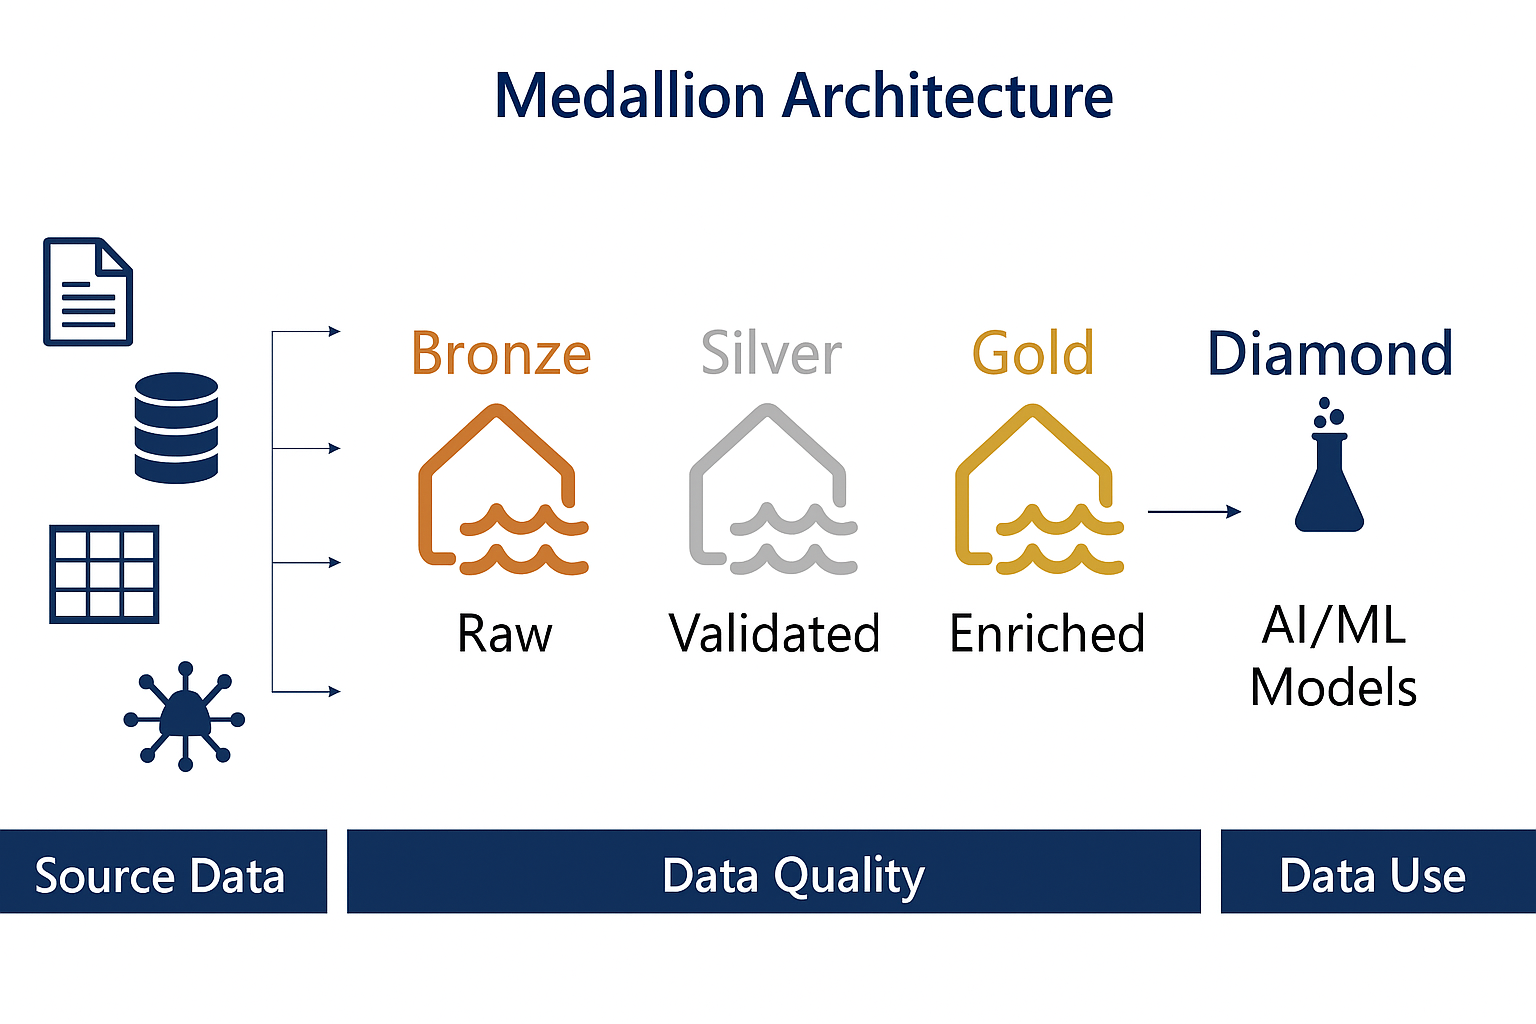
\includegraphics[width=\figwidth]{img/ChatGPT Image Sep 1, 2025, 10_13_07 AM.png}
    \caption{Architecture Medallion - Couches de données}
    \label{fig:medallion_architecture}
\end{figure}

\subsection{Pipeline ETL}
Notre pipeline ETL automatisé traite les données BVMT à travers les différentes couches :
\begin{figure}[H]
    \centering
    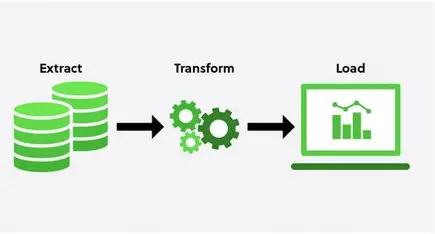
\includegraphics[width=\figwidth]{img/ETL (1).png}
    \caption{Virtual Environment}
    \label{fig:Virtual Environment}
\end{figure}

\subsubsection{Extraction (Bronze)}
\begin{itemize}
    \item Scraping automatisé des données BVMT
    \item Gestion des formats ZIP, RAR, CSV
    \item Validation de l'intégrité des données
    \item Stockage en format parquet pour l'efficacité
\end{itemize}

\subsubsection{Transformation (Silver)}
\begin{itemize}
    \item Nettoyage et validation des données
    \item Standardisation des formats
    \item Gestion des valeurs manquantes
    \item Calculs de métriques financières de base
\end{itemize}

\subsubsection{Chargement (Golden)}
\begin{itemize}
    \item Agrégation des données par période
    \item Calculs de KPIs business
    \item Optimisation des requêtes
    \item Indexation pour les performances
\end{itemize}

\subsubsection{Enrichissement (Diamond)}
\begin{itemize}
    \item Analyse statistique avancée
    \item Modèles de machine learning
    \item Prédictions et recommandations
    \item Visualisations interactives
\end{itemize}
